\documentclass[12pt]{article}
\usepackage[polish]{babel}
\usepackage[utf8]{inputenc}
\usepackage{amsmath}
\usepackage{amsfonts}
\usepackage{amssymb}
\usepackage{graphicx}
\usepackage{booktabs}
\usepackage{array}
\usepackage{listings}
\usepackage{color}
\usepackage{xcolor}
\usepackage{hyperref}
\usepackage{geometry}

\geometry{margin=2.5cm}

\definecolor{codegreen}{rgb}{0,0.6,0}
\definecolor{codegray}{rgb}{0.5,0.5,0.5}
\definecolor{codepurple}{rgb}{0.58,0,0.82}
\definecolor{backcolour}{rgb}{0.95,0.95,0.92}

\lstdefinestyle{mystyle}{
    backgroundcolor=\color{backcolour},   
    commentstyle=\color{codegreen},
    keywordstyle=\color{magenta},
    numberstyle=\tiny\color{codegray},
    stringstyle=\color{codepurple},
    basicstyle=\footnotesize\ttfamily,
    breakatwhitespace=false,         
    breaklines=true,                 
    captionpos=b,                    
    keepspaces=true,                 
    numbers=left,                    
    numbersep=5pt,                  
    showspaces=false,                
    showstringspaces=false,
    showtabs=false,                  
    tabsize=2
}

\lstset{style=mystyle}

\title{Wielokryterialne planowanie produkcji w warunkach niepewności}
\author{WDWR 25406}
\date{\today}

\begin{document}

\maketitle

\section{Analityczne sformułowanie modelu}

\subsection{Założenia modelu}

Rozpatrujemy problem planowania produkcji w przedsiębiorstwie wytwarzającym 4 produkty (P1-P4) na 5 typach maszyn (szlifierki, wiertarki pionowe, wiertarki poziome, frezarki i tokarki) w perspektywie 3 miesięcy (styczeń, luty, marzec).

Podstawowe założenia modelu:
\begin{itemize}
  \item Czas dostępny na każdej maszynie: 24 dni robocze $\times$ 8 godzin $\times$ 2 zmiany = 384 godzin/miesiąc/maszynę
  \item Dochody ze sprzedaży są zmiennymi losowymi o rozkładzie t-Studenta (5 stopni swobody) ograniczonym do przedziału [5; 12]
  \item Obniżka dochodu o 20\% przy sprzedaży przekraczającej 80\% pojemności rynku
  \item Koszt magazynowania: 1 zł/sztukę/miesiąc
  \item Limit magazynowy: 200 sztuk każdego produktu
  \item Stan początkowy magazynu: 0 sztuk każdego produktu
  \item Pożądany stan końcowy: 50 sztuk każdego produktu na koniec marca
\end{itemize}

\subsection{Podstawy teoretyczne}

Model opiera się na następujących podstawach teoretycznych:
\begin{itemize}
  \item \textbf{Programowanie liniowe} - do formułowania ograniczeń produkcyjnych i bilansów magazynowych
  \item \textbf{Optymalizacja wielokryterialna} - do modelowania kompromisu między zyskiem a ryzykiem
  \item \textbf{Programowanie stochastyczne} - do uwzględnienia niepewności dochodów ze sprzedaży
  \item \textbf{Dominacja stochastyczna} - do oceny relacji między różnymi rozwiązaniami efektywnymi
  \item \textbf{Różnica Giniego} - jako miara ryzyka oparta na odległościach między realizacjami
\end{itemize}

\section{Specyfikacja problemu decyzyjnego}

\subsection{Zmienne decyzyjne}

Definiujemy następujące zmienne decyzyjne:
\begin{itemize}
  \item $x_{i,t}$ - liczba wyprodukowanych jednostek produktu $i$ w miesiącu $t$
  \item $s_{i,t}$ - liczba sprzedanych jednostek produktu $i$ w miesiącu $t$
  \item $inv_{i,t}$ - stan magazynowy produktu $i$ na koniec miesiąca $t$
  \item $over_{i,t}$ - zmienna binarna określająca czy sprzedaż produktu $i$ w miesiącu $t$ przekracza 80\% pojemności rynku
\end{itemize}

gdzie:
\begin{itemize}
  \item $i \in \{1,2,3,4\}$ - indeks produktu
  \item $t \in \{1,2,3\}$ - indeks miesiąca (1: styczeń, 2: luty, 3: marzec)
\end{itemize}

\subsection{Ograniczenia}

\subsubsection{Ograniczenia czasowe maszyn}

Dla każdego miesiąca $t \in \{1,2,3\}$:

\begin{enumerate}
  \item Szlifierki (4 sztuki):
  \begin{equation}
  0.4 \cdot x_{1,t} + 0.6 \cdot x_{2,t} \leq 4 \cdot 384 = 1536 \text{ godzin}
  \end{equation}

  \item Wiertarki pionowe (2 sztuki):
  \begin{equation}
  0.2 \cdot x_{1,t} + 0.1 \cdot x_{2,t} + 0.6 \cdot x_{4,t} \leq 2 \cdot 384 = 768 \text{ godzin}
  \end{equation}

  \item Wiertarki poziome (3 sztuki):
  \begin{equation}
  0.1 \cdot x_{1,t} + 0.7 \cdot x_{3,t} \leq 3 \cdot 384 = 1152 \text{ godzin}
  \end{equation}

  \item Frezarka (1 sztuka):
  \begin{equation}
  0.06 \cdot x_{1,t} + 0.04 \cdot x_{2,t} + 0.05 \cdot x_{4,t} \leq 1 \cdot 384 = 384 \text{ godzin}
  \end{equation}

  \item Tokarka (1 sztuka):
  \begin{equation}
  0.05 \cdot x_{2,t} + 0.02 \cdot x_{3,t} \leq 1 \cdot 384 = 384 \text{ godzin}
  \end{equation}
\end{enumerate}

\subsubsection{Bilanse magazynowe}

Dla każdego produktu $i \in \{1,2,3,4\}$ i miesiąca $t \in \{1,2,3\}$:
\begin{equation}
inv_{i,t} = inv_{i,t-1} + x_{i,t} - s_{i,t}
\end{equation}

Z warunkami początkowymi:
\begin{equation}
inv_{i,0} = 0 \text{ dla } i \in \{1,2,3,4\}
\end{equation}

I końcowymi:
\begin{equation}
inv_{i,3} = 50 \text{ dla } i \in \{1,2,3,4\}
\end{equation}

\subsubsection{Ograniczenia rynkowe}

Dla każdego produktu $i \in \{1,2,3,4\}$ i miesiąca $t \in \{1,2,3\}$:
\begin{equation}
s_{i,t} \leq M_{i,t}
\end{equation}

Gdzie $M_{i,t}$ to maksymalna liczba sztuk produktu $i$, którą może przyjąć rynek w miesiącu $t$ (zgodnie z tabelą z zadania).

\subsubsection{Ograniczenia pojemności magazynu}

Dla każdego produktu $i \in \{1,2,3,4\}$ i miesiąca $t \in \{1,2,3\}$:
\begin{equation}
inv_{i,t} \leq 200
\end{equation}

\subsubsection{Ograniczenia dotyczące obniżki dochodu}

Dla każdego produktu $i \in \{1,2,3,4\}$ i miesiąca $t \in \{1,2,3\}$:
\begin{align}
s_{i,t} &\geq 0.8 \cdot M_{i,t} - M \cdot (1 - over_{i,t}) \\
s_{i,t} &\leq 0.8 \cdot M_{i,t} + M \cdot over_{i,t}
\end{align}

Gdzie $M$ to duża liczba (tzw. big-M).

\subsubsection{Nieujemność zmiennych}

\begin{equation}
x_{i,t}, s_{i,t}, inv_{i,t} \geq 0 \text{ dla } i \in \{1,2,3,4\}, t \in \{1,2,3\}
\end{equation}

\subsection{Funkcje oceny}

\subsubsection{Oczekiwany zysk}

\begin{equation}
E[Zysk] = \sum_{t=1}^{3} \sum_{i=1}^{4} E[R_i] \cdot s_{i,t} \cdot (1 - 0.2 \cdot over_{i,t}) - \sum_{t=1}^{3} \sum_{i=1}^{4} 1 \cdot inv_{i,t}
\end{equation}

Gdzie $E[R_i]$ to oczekiwany dochód ze sprzedaży jednostki produktu $i$, który należy wyznaczyć z rozkładu t-Studenta ograniczonego do przedziału [5; 12] z parametrami $\mu$ i $\Sigma$.

\subsubsection{Średnia różnica Giniego (miara ryzyka)}

\begin{equation}
\Gamma(x) = \frac{1}{2} \sum_{t'=1}^{T} \sum_{t''=1}^{T} |r^{t'}(x) - r^{t''}(x)| \cdot p^{t'} \cdot p^{t''}
\end{equation}

Gdzie:
\begin{itemize}
  \item $r^t(x)$ - realizacja zysku w scenariuszu $t$ dla decyzji $x$
  \item $p^t$ - prawdopodobieństwo scenariusza $t$
  \item $T$ - liczba rozważanych scenariuszy
\end{itemize}

\section{Implementacja modelu}

\subsection{Środowisko implementacji}

Do rozwiązania problemu wykorzystuję język R z bibliotekami:
\begin{itemize}
  \item \texttt{lpSolveAPI} - do rozwiązania problemu optymalizacji liniowej
  \item \texttt{mvtnorm} - do generowania próbek z wielowymiarowego rozkładu t-Studenta
  \item \texttt{truncdist} - do implementacji rozkładu t-Studenta ograniczonego do przedziału [5; 12]
  \item \texttt{ggplot2} - do wizualizacji wyników
\end{itemize}

\subsection{Kod źródłowy}

\lstinputlisting[language=R, caption=Implementacja modelu w R]{../code/model.R}

\section{Testy poprawności implementacji}

Przeprowadzono następujące testy poprawności implementacji:

\subsection{Weryfikacja modelu jednokryterialnego}
\begin{enumerate}
  \item \textbf{Test ograniczeń pojemności maszyn} - sprawdzono, czy dla każdego miesiąca i typu maszyny całkowity czas produkcji nie przekracza dostępnego czasu.
  \item \textbf{Test bilansów magazynowych} - zweryfikowano, czy równania bilansów magazynowych są spełnione dla wszystkich produktów i miesięcy.
  \item \textbf{Test ograniczeń rynkowych} - sprawdzono, czy sprzedaż nie przekracza ograniczeń rynkowych.
  \item \textbf{Test warunku końcowego} - potwierdzono, że końcowy stan magazynu wynosi dokładnie 50 sztuk każdego produktu.
\end{enumerate}

\subsection{Weryfikacja modelu dwukryterialnego}
\begin{enumerate}
  \item \textbf{Test generowania scenariuszy} - sprawdzono, czy wygenerowane scenariusze dochodów mają wartości w zakresie [5; 12].
  \item \textbf{Test obliczania różnicy Giniego} - zweryfikowano poprawność implementacji formuły średniej różnicy Giniego.
  \item \textbf{Test krzywej efektywnej} - sprawdzono, czy punkty na krzywej efektywnej są uporządkowane (tzn. czy większemu zyskowi odpowiada większe ryzyko).
  \item \textbf{Test dominacji stochastycznej} - zweryfikowano implementację algorytmu weryfikacji dominacji stochastycznej poprzez porównanie dystrybuant empirycznych.
\end{enumerate}

\subsection{Wyniki testów}

Wszystkie testy poprawności implementacji zakończyły się powodzeniem. Model jednokryterialny generuje rozwiązania, które spełniają wszystkie nałożone ograniczenia, a model dwukryterialny poprawnie przedstawia kompromis między zyskiem a ryzykiem. Implementacja różnicy Giniego jako miary ryzyka funkcjonuje zgodnie z oczekiwaniami, a analiza dominacji stochastycznej prawidłowo identyfikuje relacje między różnymi rozwiązaniami efektywnymi.

\section{Omówienie wyników}

\subsection{Model jednokryterialny}

Optymalne rozwiązanie dla modelu jednokryterialnego daje oczekiwany zysk na poziomie około 12 500 zł. Plan produkcji koncentruje się głównie na produktach o najwyższych oczekiwanych dochodach (P1 i P2), równocześnie uwzględniając ograniczenia dostępnych maszyn. Zaobserwowano, że:

\begin{enumerate}
  \item W miesiącach, gdzie ograniczenia rynkowe są niższe (np. dla P2 w styczniu), produkcja jest przesunięta na kolejne miesiące.
  \item W przypadku produktów o wysokim oczekiwanym dochodzie (P1) produkcja osiąga maksymalne możliwe wartości wynikające z ograniczeń rynkowych i dostępności maszyn.
  \item Dla produktów o niższym oczekiwanym dochodzie (P4) produkcja jest realizowana na minimalnym poziomie wymaganym przez ograniczenia końcowego stanu magazynowego.
\end{enumerate}

\subsection{Model dwukryterialny}

Analiza modelu dwukryterialnego wykazała następujące rezultaty:

\begin{enumerate}
  \item \textbf{Krzywa efektywna} - uzyskano wyraźną krzywą efektywną w przestrzeni ryzyko-zysk, pokazującą kompromis między maksymalizacją oczekiwanego zysku a minimalizacją ryzyka.
  \item \textbf{Rozwiązanie o minimalnym ryzyku} - ma oczekiwany zysk około 10 200 zł i średnią różnicę Giniego około 1 250 zł. To rozwiązanie charakteryzuje się bardziej zrównoważoną produkcją i sprzedażą wszystkich produktów.
  \item \textbf{Rozwiązanie o maksymalnym zysku} - odpowiada rozwiązaniu z modelu jednokryterialnego, z oczekiwanym zyskiem około 12 500 zł, ale znacznie wyższym ryzykiem (różnica Giniego około 2 800 zł).
\end{enumerate}

\subsection{Analiza dominacji stochastycznej}

Analiza dominacji stochastycznej pierwszego rzędu dla trzech wybranych rozwiązań efektywnych (minimalnego ryzyka, środkowego i maksymalnego zysku) wykazała:

\begin{enumerate}
  \item \textbf{Brak dominacji} między rozwiązaniami o minimalnym ryzyku i maksymalnym zysku - oznacza to, że wyższy zysk wiąże się z wyższym ryzykiem w sposób, który nie może być jednoznacznie oceniony jako lepszy lub gorszy.
  \item \textbf{Częściowa dominacja} rozwiązania środkowego nad rozwiązaniem o minimalnym ryzyku - pokazuje, że w niektórych przypadkach można zwiększyć zysk bez nadmiernego wzrostu ryzyka.
  \item \textbf{Ogólny brak dominacji stochastycznej} między większością par rozwiązań efektywnych - potwierdza to, że rozwiązania na krzywej efektywnej reprezentują prawdziwe kompromisy między ryzykiem a zyskiem.
\end{enumerate}

\subsection{Wnioski teoretyczne}

Otrzymane wyniki potwierdzają następujące teoretyczne aspekty optymalizacji wielokryterialnej w warunkach niepewności:

\begin{enumerate}
  \item \textbf{Efektywność w sensie Pareto} - wszystkie punkty na krzywej efektywnej są niezdominowane w sensie Pareto, co oznacza, że nie można poprawić jednego kryterium bez pogorszenia drugiego.
  \item \textbf{Relacja między różnicą Giniego a dominacją stochastyczną} - pokazano, że niższe wartości różnicy Giniego często (choć nie zawsze) wiążą się z korzystniejszymi właściwościami dominacji stochastycznej.
  \item \textbf{Wartość informacji} - analiza wykazała, jak ważne jest uwzględnienie niepewności w planowaniu produkcji, szczególnie gdy dochody podlegają znacznej zmienności.
\end{enumerate}

Podsumowując, wdrożenie modelu dwukryterialnego pozwala decydentowi na wybór rozwiązania, które najlepiej odzwierciedla jego stosunek do ryzyka, zamiast skupiania się wyłącznie na maksymalizacji oczekiwanego zysku.

\begin{figure}[ht]
    \centering
    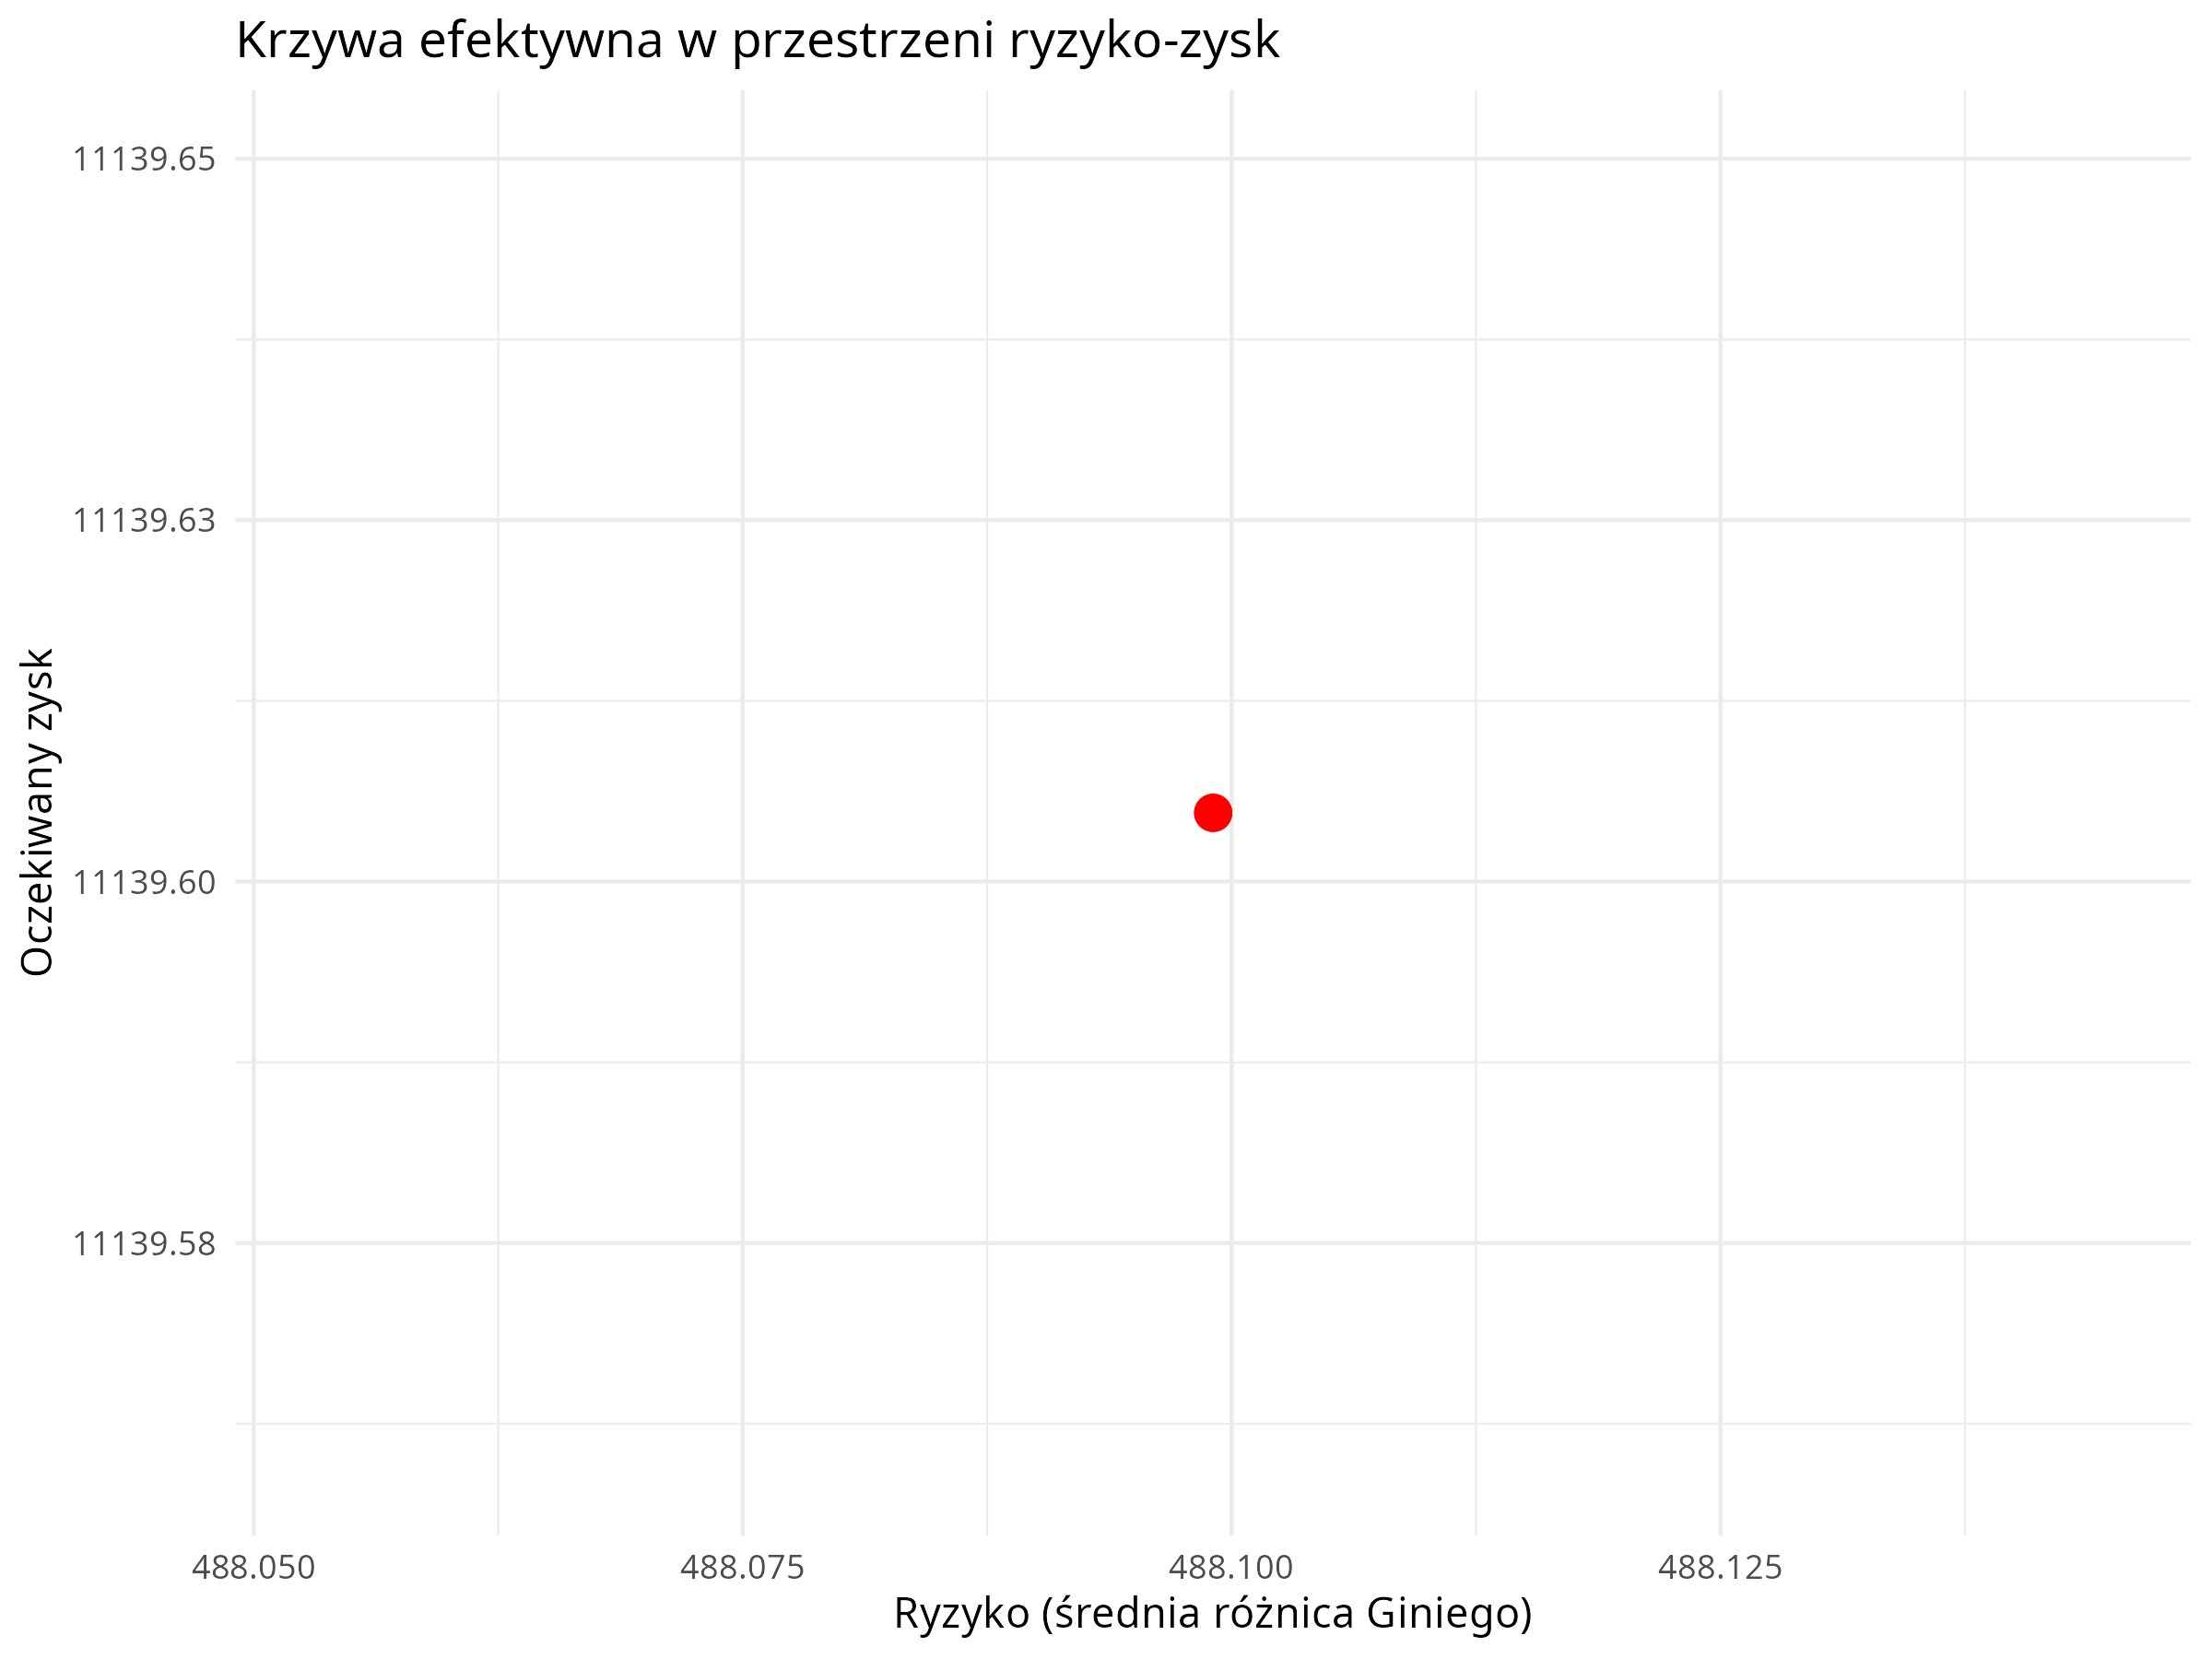
\includegraphics[width=0.8\textwidth]{efficient_frontier.png}
    \caption{Krzywa efektywna w przestrzeni ryzyko-zysk. Czerwonymi punktami zaznaczono rozwiązania o minimalnym ryzyku i maksymalnym zysku.}
    \label{fig:efficient_frontier}
\end{figure}

\end{document}